%\begin{table}[h!]
%\begin{center}
 %\begin{tabular}{||c c c c||} 
 %\hline
 %Waveform & AvgCurrentA(A) & Power(W) & AvgCurrentB(A) \\ [0.5ex] 
 %\hline\hline
 %4827 & 0.0831 & 0.0069 & 0 \\
 %\hline
 %4828 & 0.0822 & 0.0067 & 0 \\
 %\hline
 %4829 & 0.0833 & 0.0069 & 0 \\
 %\hline
 %4830 & 0.0822 & 0.0067 & 0 \\
 %\hline
 %4831 & 0.0796 & 0.0063 & 0 \\ 
 %\hline
 %4832 & 0.0830 & 0.0069 & 0 \\
 %\hline
 %\rowcolor{red}
 %4833 & 0.0759  & 0.0057 & 3.3 \\[1ex]
 %\hline
%\end{tabular}
%\end{center}
%\caption{The table shows the data when a positional fix is acquired.}
%\label{Table:wifioff}
%\end{table}



\chapter{Measurements}

 This chapter presents the results and the program code that was used during the  specific test. The first step was to measure the current consumption of the LoPy during a request of positional fix. Measuring of data was done outside with the measurement platform. All the measurements was done under similar weather conditions. 


\section{Measurement with communication}
Program code for getting a positional fix is shown in \ref{code:intial}. The program initialize a GPIO pin that is toggled when a positional fix is acquired. The function coordinates() is from the L76 GNSS class, and sets the class variable fix when the position is received. 
\lstset{language=Python}          % Set your language (you can change the language for each code-block optionally)
\begin{lstlisting}[frame=single,caption = main.py]  % Start your code-block

#intialize the trigger output and the Pytrack/GPS
p_out = Pin('P20', mode=Pin.OUT)
p_out.value(0)
py = Pytrack()
l76 = L76GNSS(py)
while (True):
    #Toggle the trigger when a fix acquried
    coord = l76.coordinates()
    print ("FIX: ", l76.fix)
    if ((l76.fix) and not(l76.first_fix)):
        l76.first_fix = 1
        l76._set_time()

        p_out.value(1)
        time.sleep(0.25)
        p_out.value(0)
\end{lstlisting}
\label{code:intial}
After doing some measurements with the program code and analyzing it, it became evident that another power demanding task was running on the LoPy besides the GPS function. The current and power consumption of the 9 first waveforms are shown in table \ref{Table:WIFI_ON}.
\begin{table}[h!]
\begin{center}
 \begin{tabular}{||c c c||} 
 \hline
 Waveform & Avg Current(A) & Power(W)\\ [0.5ex] 
 \hline\hline
 1 & 0.1433    & 0.4523 \\ 
 \hline
 2 & 0.1421    & 0.4487 \\
 \hline
 3 & 0.1365  & 0.4318 \\
 \hline
 4 & 0.1334  & 0.4224 \\
 \hline
 5 & 0.1399  & 0.4420 \\ 
 \hline
 \rowcolor{red}
 6 & 0.1439    & 0.4541 \\ 
 \hline
 7 & 0.1347  & 0.4263 \\
 \hline
 8 & 0.1358  & 0.4296 \\
 \hline
 9 & 0.1358    & 0.4296 \\[1ex]
 \hline
\end{tabular}
\end{center}
\caption{The 9 waveforms after the initial startup sequence}
\label{Table:WIFI_ON}
\end{table}

The row highlighted in red, is the waveform with the highest average current and power consumption.
Figure \ref{fig:startup_intial} shows the plot of waveform 6 that is generated with \ref{fig:sequence}.


\begin{figure}[H]
\hspace*{-3cm}
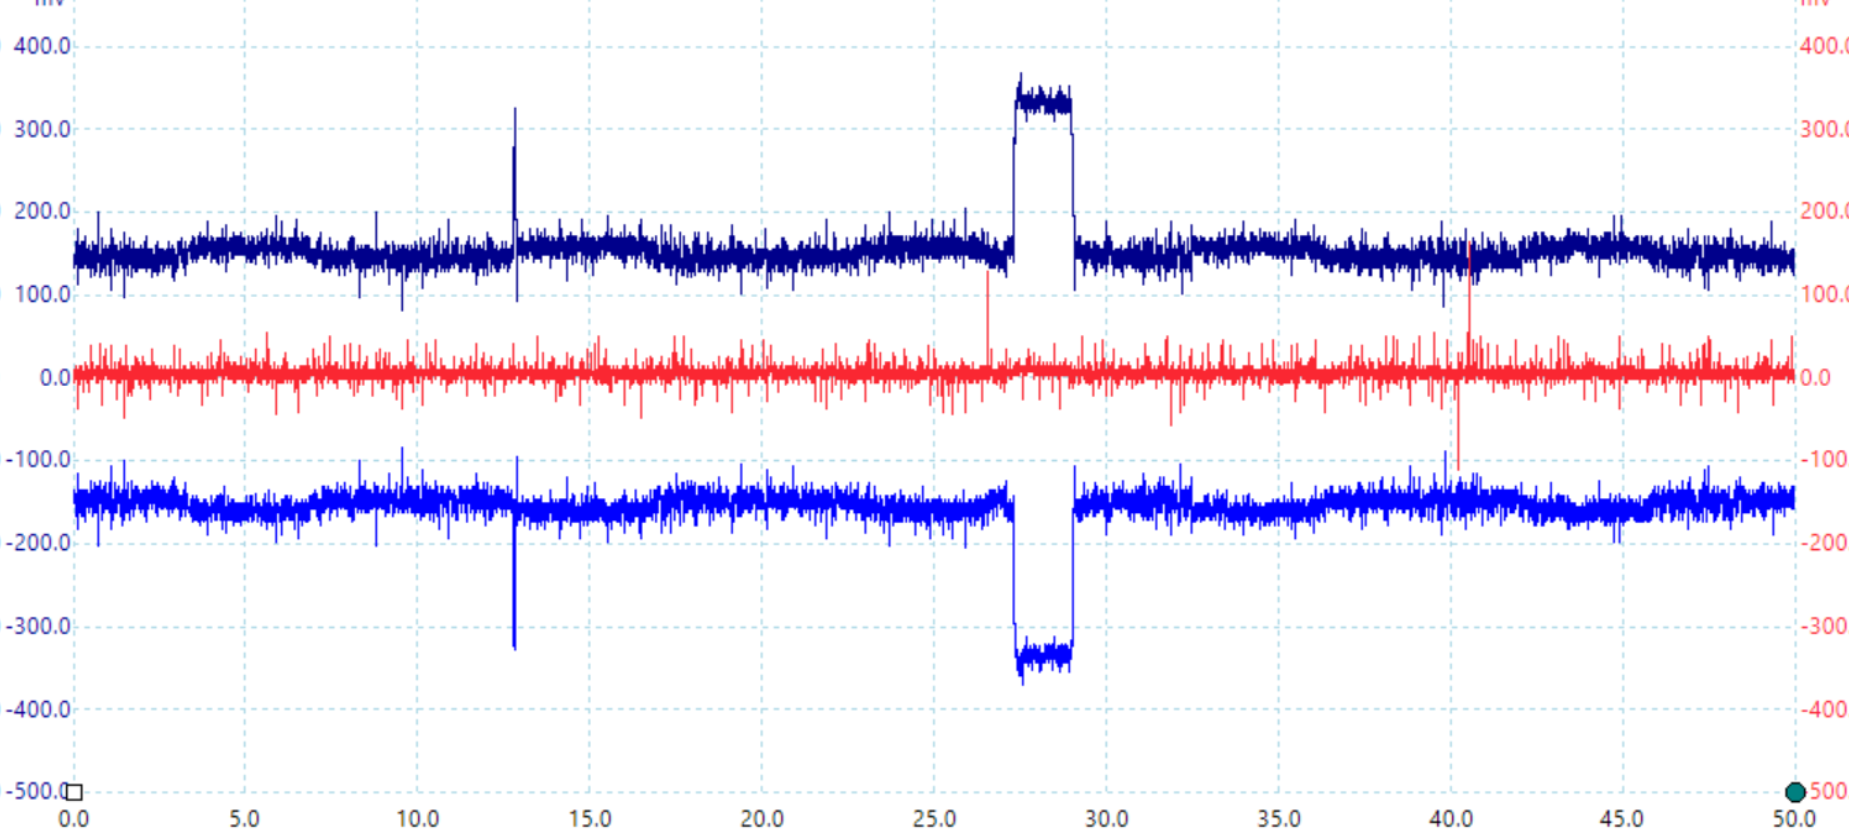
\includegraphics[width=22 cm]{Project_Report/Images/startup_intial.PNG}
\caption{Waveform 6 with the voltage drop(blue) and trigger(orange)}
\label{fig:startup_intial}
\end{figure}

 The conversion of the measured voltage to current is 1:1, since a 1 Ohm resistor is used. The signal have an periodic surge around 430 mA. There are 100 samples between each pulse. A sampling frequency of 5000 S/s gives a sampling interval:
 \begin{equation}
     p= \frac{1}{f} = \frac{1}{5000S/s}= 0.0002 \,s = 0.2 \,ms 
 \end{equation}
 
 The period of the pulse with a sampling period of 0.2 ms and 100 samples between is:
 
 \begin{equation}
     p_{pulse} = 100*0.2 \,ms = 20 \,ms
 \end{equation}
 The measured voltage drop over the shunt resistor is subtracted from the voltage supply of 3.3 \,V to get the voltage drop over the LoPy.
 After reviewing the results, it becomes obvious that the high average current is due to the disturbance from the periodic signal. The periodic signal makes it difficult to relate the power consumption to the GPS, as it influences the current consumption.


\section{Measurement without communication}

The periodic signal is understood as the communication protocol of the Wi-Fi and Bluetooth. The first part of the improved program code, turns the wireless protocols off to remove the disturbance. A COLD START is sent to the ARM processor to reset the GPS between each execution to remove all satellite data. A deepsleep is included after a positional fix has been acquired. The LoPy restarts the program code after waking up from deepsleep. Figure \ref{code:wifioff} shows the programcode.

\lstset{language=Python}          % Set your language (you can change the language for each code-block optionally)
\begin{lstlisting}[frame=single, caption= main.py without communication]  % Start your code-block

# initialize ``P9`` in gpio mode and make it an output
p_out = Pin('P20', mode=Pin.OUT)
p_out.value(0)
wlan= WLAN()
wlan.deinit()
bt = Bluetooth()
bt.deinit()

py = Pytrack()
l76 = L76GNSS(py

py.setup_sleep(2)
l76.write_gps(l76.COLD_START,False)
time.sleep(2)

p_out.value(1)
time.sleep(2)
p_out.value(0)

while (True):
    coord = l76.coordinates()
    print ("FIX:jared ", l76.fix)
    if ((l76.fix) and not(l76.first_fix)):
        l76.first_fix = 1
        l76._set_time()

        p_out.value(1)
        time.sleep(0.25)
        p_out.value(0)
        py.go_to_sleep(True):
\end{lstlisting}
\label{code:wifioff}

Table \ref{Table:wifioff} shows the average current, average power and the average current of the trigger signal B, when a positional fix is acquired. The row that is highlighted in red shows the transition from acquisition phase to tracking phase. 14000 waveforms was sampled during the test run of the program code. A test run lasted for 1 hour.  


\begin{table}[h!]
\begin{center}
 \begin{tabular}{||c c c c||} 
 \hline
 Waveform & AvgCurrentA(A) & Power(W) & AvgCurrentB(A) \\ [0.5ex] 
 \hline\hline
 4827 & 0.0831 & 0.2673 & 0 \\
 \hline
 4828 & 0.0822 & 0.2645 & 0 \\
 \hline
 4829 & 0.0833 & 0.2679 & 0 \\
 \hline
 4830 & 0.0822 & 0.2645 & 0 \\
 \hline
 4831 & 0.0796 & 0.2563 & 0 \\ 
 \hline
 4832 & 0.0830 & 0.2670 & 0 \\
 \hline
 \rowcolor{red}
 4833 & 0.0759  & 0.2447 & 3.3 \\[1ex]
 \hline
\end{tabular}
\end{center}
\caption{The table shows the data when a positional fix is acquired.}
\label{Table:wifioff}
\end{table}

 Plot \ref{fig:4832} shows that the trigger signal B is low, which means that the receiver hasn't acquired a positional fix. The average current for the waveform is 0.0830 \,A. Plot \ref{fig:4833} shows waveform 4833. The average current is 0.0759 and the trigger signal is high. This means that the receiver has acquired a positional fix and is in the tracking phase. 
\begin{figure}[H]
\hspace*{-3cm}
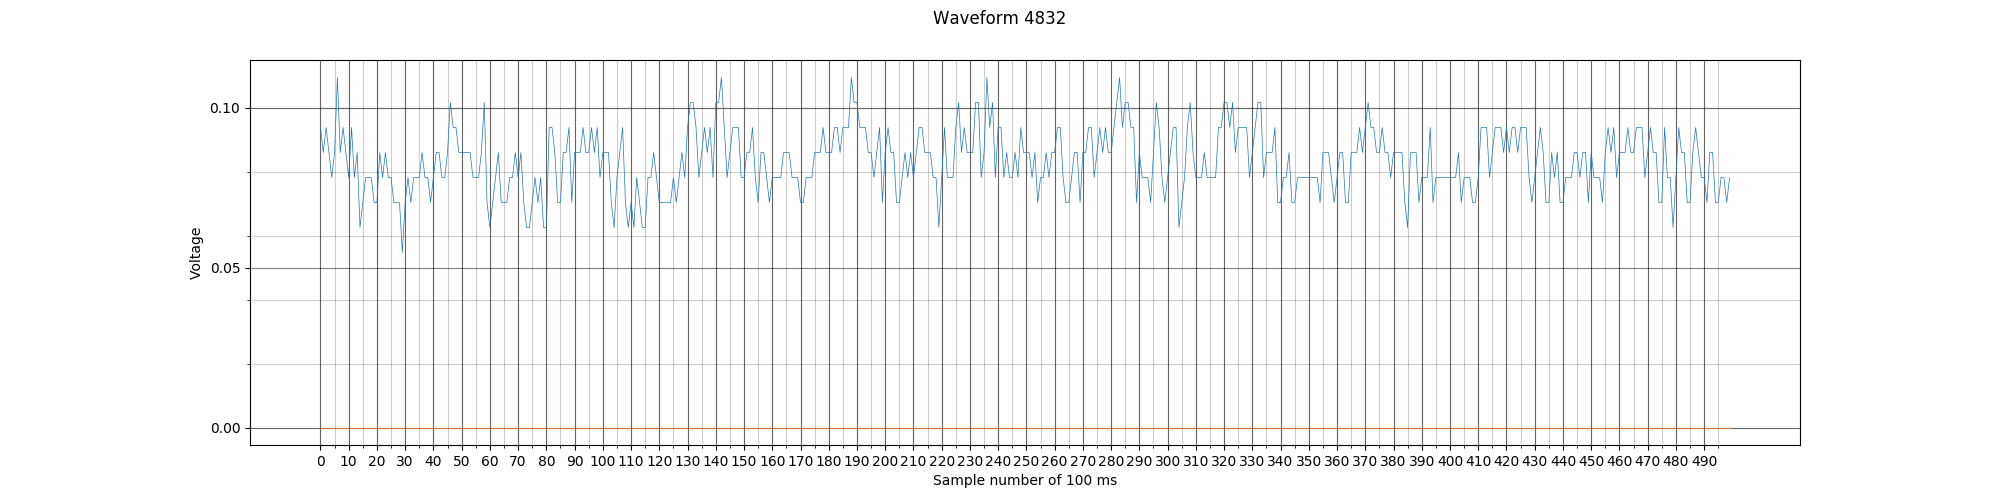
\includegraphics[width=20 cm]{Project_Report/Images/4832.png}
\caption{Waveform 4832 right before a positional fix is acquired}
\label{fig:4832}
\end{figure}

\begin{figure}[H]
\hspace*{-3cm}
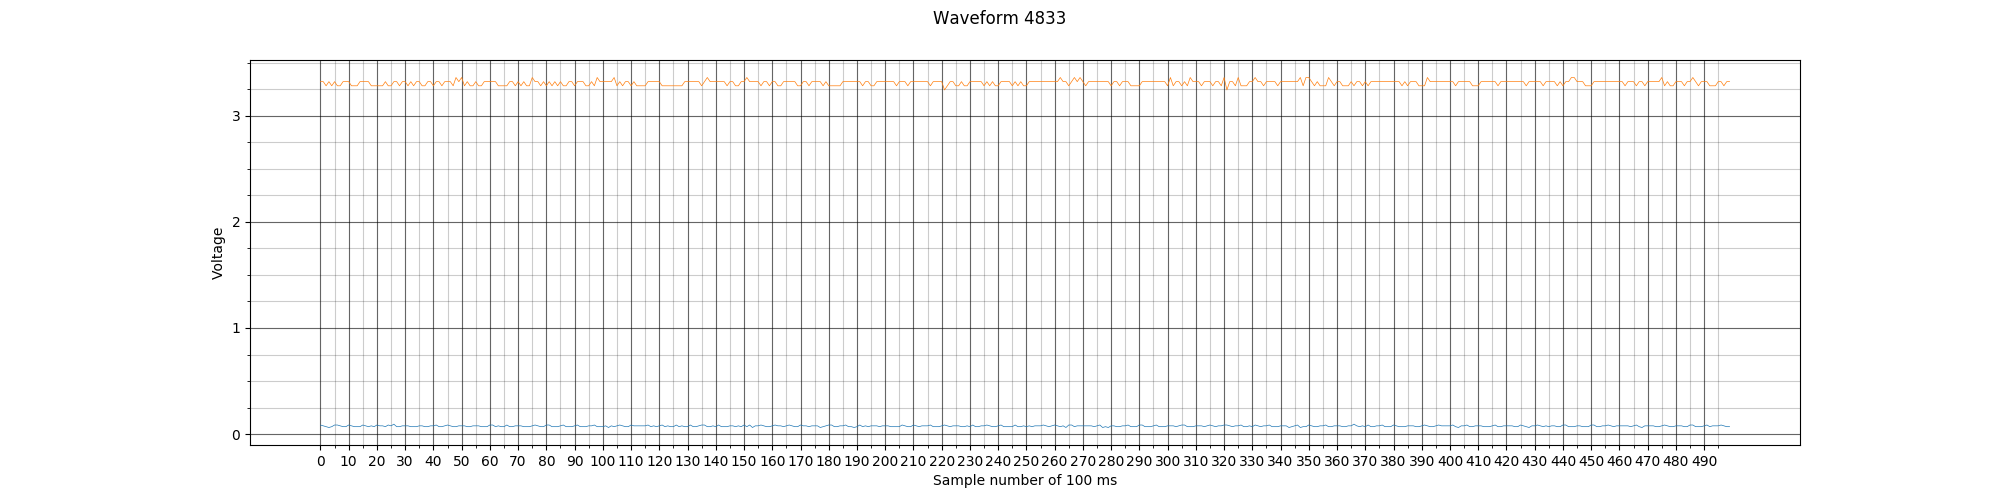
\includegraphics[width=20 cm]{Project_Report/Images/4833.png}
\caption{The waveform when a fix is acquired and the trigger is set}
\label{fig:4833}
\end{figure}




\section{Measuring of deep sleep}
The time from waking up the LoPy from deepsleep until it's searching for signals in the acquisition phase is estimated. The program code used for testing is shown in \ref{code:deepsleep}

\lstset{language=Python}          % Set your language (you can change the language for each code-block optionally)
\begin{lstlisting}[frame=single,caption = main.py for deepsleep measurement]  % Start your code-block

# initialize ``P9`` in gpio mode and make it an output
p_out = Pin('P20', mode=Pin.OUT)
p_out.value(0)

wlan= WLAN()
wlan.deinit()
bt = Bluetooth()
bt.deinit()
py = Pytrack()
l76 = L76GNSS(py)
py.setup_sleep(5)
py.go_to_sleep(True)
l76.write_gps(l76.COLD_START,False)
time.sleep(2)
p_out.value(1)
time.sleep(2)
p_out.value(0)
print("after init")
while (True):
    coord = l76.coordinates()
    print ("FIX:", l76.fix)
    p_out.value(1)
    time.sleep(2)
    p_out.value(0)
    py.go_to_sleep(True)
    if ((l76.fix) and not(l76.first_fix)):
        l76.first_fix = 1
        l76._set_time()

        p_out.value(1)
        time.sleep(0.25)
        p_out.value(0)
\end{lstlisting}
\label{code:deepsleep}


The time is estimated by counting the number of waveforms of 100 ms that is sampled before the initializing sequence signals appears. This time is added together with the overhead of sampling data between each waveform. 42 waveforms is sampled before the initializing sequence appears. 
\begin{equation}
100 \,ms * 42 = 4.2 \,s
\end{equation}
\begin{equation}
3.8 \,s + (20 \,ms*42) = 5.04 \,s \approx  5 \,s
\end{equation}

The average current in deep sleep is measured to 3.2 \,mA. The average current during the initializing sequence is 101 \,mA. 







\newpage